\chapter{Geometrija}

\index{geometrija}

U geometrijskim zadacima često je izazovno
pronaći način pristupa zadatku takav da se
rješenje zadatka može jednostavno implementirati
i da je broj posebnih slučajeva malen.

Kao primjer, razmotrimo zadatak u kojem
su nam zadani vrhovi četverokuta
(mnogokuta koji ima četiri vrha),
a naš je zadatak izračunati njegovu površinu.
Na primjer, mogući ulaz za taj zadatak izgleda ovako:

\begin{center}
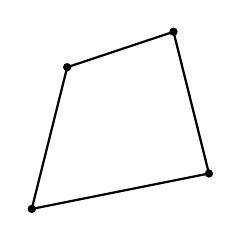
\begin{tikzpicture}[scale=0.45]

\draw[fill] (6,2) circle [radius=0.1];
\draw[fill] (5,6) circle [radius=0.1];
\draw[fill] (2,5) circle [radius=0.1];
\draw[fill] (1,1) circle [radius=0.1];
\draw[thick] (6,2) -- (5,6) -- (2,5) -- (1,1) -- (6,2);
\end{tikzpicture}
\end{center}
Jedan način pristupa zadatku jest podijeliti
četverokut na dva trokuta pravcem
između dva nasuprotna vrha:
\begin{center}
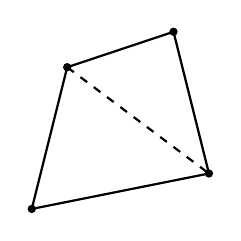
\begin{tikzpicture}[scale=0.45]

\draw[fill] (6,2) circle [radius=0.1];
\draw[fill] (5,6) circle [radius=0.1];
\draw[fill] (2,5) circle [radius=0.1];
\draw[fill] (1,1) circle [radius=0.1];

\draw[thick] (6,2) -- (5,6) -- (2,5) -- (1,1) -- (6,2);
\draw[dashed,thick] (2,5) -- (6,2);
\end{tikzpicture}
\end{center}
Nakon toga dovoljno je zbrojiti površine
trokuta.
Površinu trokuta možemo izračunati,
na primjer, pomoću \key{Heronove formule}
%\footnote{Heron of Alexandria (c. 10--70) was a Greek mathematician.}
\[ \sqrt{s (s-a) (s-b) (s-c)},\]
gdje su $a$, $b$ i $c$ duljine
stranica trokuta, a
$s=(a+b+c)/2$.
\index{Heronova formula}

Ovo je jedan mogući način rješavanja zadatka,
ali postoji jedna zamka:
kako podijeliti četverokut na trokute?
Pokazuje se da ponekad ne možemo jednostavno odabrati
bilo koja dva nasuprotna vrha.
Na primjer, u sljedećoj situaciji
pravac podjele nalazi se \emph{izvan} četverokuta:
\begin{center}
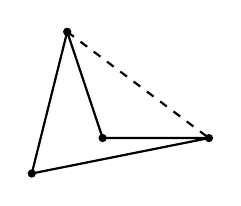
\begin{tikzpicture}[scale=0.45]

\draw[fill] (6,2) circle [radius=0.1];
\draw[fill] (3,2) circle [radius=0.1];
\draw[fill] (2,5) circle [radius=0.1];
\draw[fill] (1,1) circle [radius=0.1];
\draw[thick] (6,2) -- (3,2) -- (2,5) -- (1,1) -- (6,2);

\draw[dashed,thick] (2,5) -- (6,2);
\end{tikzpicture}
\end{center}
Međutim, drugi način povlačenja pravca funkcionira:
\begin{center}
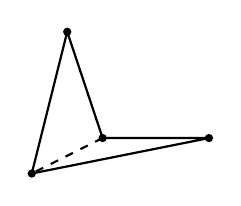
\begin{tikzpicture}[scale=0.45]

\draw[fill] (6,2) circle [radius=0.1];
\draw[fill] (3,2) circle [radius=0.1];
\draw[fill] (2,5) circle [radius=0.1];
\draw[fill] (1,1) circle [radius=0.1];
\draw[thick] (6,2) -- (3,2) -- (2,5) -- (1,1) -- (6,2);

\draw[dashed,thick] (3,2) -- (1,1);
\end{tikzpicture}
\end{center}
Čovjeku je jasno koji je pravac ispravan
izbor, ali je situacija teška za računalo.
                           
Ipak, pokazuje se da zadatak možemo riješiti
drugom metodom koja je programeru prikladnija.
Naime, postoji opća formula
\[x_1y_2-x_2y_1+x_2y_3-x_3y_2+x_3y_4-x_4y_3+x_4y_1-x_1y_4,\]
koja računa površinu četverokuta
čiji su vrhovi
$(x_1,y_1)$,
$(x_2,y_2)$,
$(x_3,y_3)$ i
$(x_4,y_4)$.
Tu je formulu lako implementirati, nema posebnih
slučajeva, a možemo je čak i poopćiti
na \emph{sve} mnogokute.

\section{Kompleksni brojevi}

\index{kompleksni broj}
\index{točka}
\index{vektor}

\key{Kompleksni broj} je broj oblika $x+y i$,
gdje je $i = \sqrt{-1}$ \key{imaginarna jedinica}.
Geometrijska interpretacija kompleksnog broja jest
da on predstavlja dvodimenzionalnu točku $(x,y)$
ili vektor od ishodišta do točke $(x,y)$.

Na primjer, $4+2i$ odgovara
sljedećoj točki i vektoru:

\begin{center}
\begin{tikzpicture}[scale=0.45]

\draw[->,thick] (-5,0)--(5,0);
\draw[->,thick] (0,-5)--(0,5);

\draw[fill] (4,2) circle [radius=0.1];
\draw[->,thick] (0,0)--(4-0.1,2-0.1);

\node at (4,2.8) {$(4,2)$};
\end{tikzpicture}
\end{center}

\index{complex@\texttt{complex}}

C++ klasa za kompleksne brojeve \texttt{complex}
korisna je pri rješavanju geometrijskih zadataka.
Pomoću te klase možemo prikazati točke i vektore
kao kompleksne brojeve, a klasa sadrži alate
koji su korisni u geometriji.

U sljedećem kodu \texttt{C} je tip
koordinate, a \texttt{P} je tip točke ili vektora.
Osim toga, kod definira makroe \texttt{X} i \texttt{Y}
kojima se možemo služiti za dohvaćanje x i y koordinate.

\begin{lstlisting}
typedef long long C;
typedef complex<C> P;
#define X real()
#define Y imag()
\end{lstlisting}

Na primjer, sljedeći kod definira točku $p=(4,2)$
i ispisuje njezinu x i y koordinatu:

\begin{lstlisting}
P p = {4,2};
cout << p.X << " " << p.Y << "\n"; // 4 2
\end{lstlisting}

Sljedeći kod definira vektore $v=(3,1)$ i $u=(2,2)$,
a nakon toga računa sumu $s=v+u$.

\begin{lstlisting}
P v = {3,1};
P u = {2,2};
P s = v+u;
cout << s.X << " " << s.Y << "\n"; // 5 3
\end{lstlisting}

U praksi je
prikladan tip koordinate obično
\texttt{long long} (cijeli broj) ili \texttt{long double}
(realni broj).
Dobra je ideja koristiti cijele brojeve kad god je to moguće,
jer su računanja s cijelim brojevima točna.
Ako su potrebni realni brojevi,
pri uspoređivanju brojeva treba uzeti u obzir
pogreške zaokruživanja.
Siguran način provjere jesu li realni brojevi $a$ i $b$ jednaki
jest usporediti ih pomoću $|a-b|<\epsilon$,
gdje je $\epsilon$ malen broj (na primjer, $\epsilon=10^{-9}$).

\subsubsection*{Funkcije}

U sljedećim primjerima tip koordinate je
\texttt{long double}.

Funkcija $\texttt{abs}(v)$ računa duljinu
$|v|$ vektora $v=(x,y)$
pomoću formule $\sqrt{x^2+y^2}$.
Funkcija se može koristiti i za
računanje udaljenosti između točaka
$(x_1,y_1)$ i $(x_2,y_2)$,
jer je ta udaljenost jednaka duljini
vektora $(x_2-x_1,y_2-y_1)$.

Sljedeći kod računa udaljenost
između točaka $(4,2)$ i $(3,-1)$:
\begin{lstlisting}
P a = {4,2};
P b = {3,-1};
cout << abs(b-a) << "\n"; // 3.16228
\end{lstlisting}

Funkcija $\texttt{arg}(v)$ računa
kut vektora $v=(x,y)$ u odnosu na os x.
Funkcija daje kut u radijanima,
pri čemu $r$ radijana odgovara $180 r/\pi$ stupnjeva.
Kut vektora koji pokazuje udesno iznosi 0,
a kutovi se smanjuju u smjeru kazaljke na satu i povećavaju
u smjeru suprotnom od kazaljke na satu.

Funkcija $\texttt{polar}(s,a)$ konstruira vektor
čija je duljina $s$ i koji pokazuje u smjeru kuta $a$.
Vektor možemo zarotirati za kut $a$
tako da ga pomnožimo vektorom duljine 1 i kuta $a$.

Sljedeći kod računa kut
vektora $(4,2)$, rotira ga za $1/2$ radijana
u smjeru suprotnom od kazaljke na satu, i zatim ponovno računa kut:

\begin{lstlisting}
P v = {4,2};
cout << arg(v) << "\n"; // 0.463648
v *= polar(1.0,0.5);
cout << arg(v) << "\n"; // 0.963648
\end{lstlisting}

\section{Točke i pravci}

\index{vektorski produkt}

\key{Vektorski produkt} $a \times b$ vektora
$a=(x_1,y_1)$ i $b=(x_2,y_2)$ računa se
pomoću formule $x_1 y_2 - x_2 y_1$.
Vektorski produkt govori nam skreće li $b$
ulijevo (pozitivna vrijednost), ne skreće (nula)
ili skreće udesno (negativna vrijednost)
kada je postavljen neposredno nakon $a$.

Sljedeća slika ilustrira navedene slučajeve:
\begin{center}
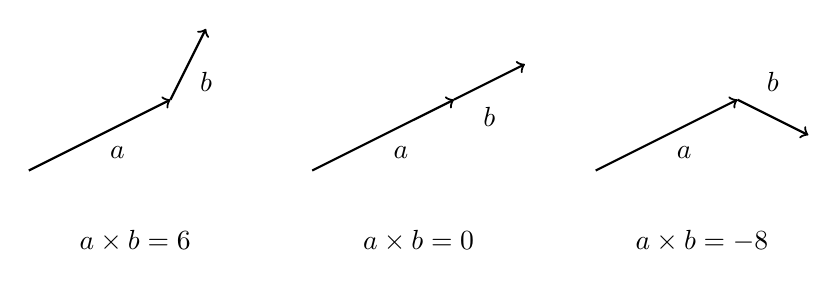
\begin{tikzpicture}[scale=0.45]

\draw[->,thick] (0,0)--(4,2);
\draw[->,thick] (4,2)--(4+1,2+2);

\node at (2.5,0.5) {$a$};
\node at (5,2.5) {$b$};

\node at (3,-2) {$a \times b = 6$};

\draw[->,thick] (8+0,0)--(8+4,2);
\draw[->,thick] (8+4,2)--(8+4+2,2+1);

\node at (8+2.5,0.5) {$a$};
\node at (8+5,1.5) {$b$};

\node at (8+3,-2) {$a \times b = 0$};

\draw[->,thick] (16+0,0)--(16+4,2);
\draw[->,thick] (16+4,2)--(16+4+2,2-1);

\node at (16+2.5,0.5) {$a$};
\node at (16+5,2.5) {$b$};

\node at (16+3,-2) {$a \times b = -8$};
\end{tikzpicture}
\end{center}

\noindent
Na primjer, u prvom slučaju
$a=(4,2)$ i $b=(1,2)$.
Sljedeći kod računa vektorski produkt
pomoću klase \texttt{complex}:

\begin{lstlisting}
P a = {4,2};
P b = {1,2};
C p = (conj(a)*b).Y; // 6
\end{lstlisting}

Gornji kod radi zato što
funkcija \texttt{conj} mijenja predznak y koordinate
vektora,
pa kada se vektori $(x_1,-y_1)$ i $(x_2,y_2)$
pomnože, y koordinata
rezultata iznosi $x_1 y_2 - x_2 y_1$.

\subsubsection{Položaj točke}

Vektorske produkte možemo koristiti za provjeru
nalazi li se točka s lijeve ili desne
strane pravca.
Pretpostavimo da pravac prolazi točkama
$s_1$ i $s_2$, da gledamo od $s_1$
prema $s_2$ i da je točka $p$.

Na primjer, na sljedećoj slici
$p$ je s lijeve strane pravca:
\begin{center}
\begin{tikzpicture}[scale=0.45]
\draw[dashed,thick,->] (0,-3)--(12,6);
\draw[fill] (4,0) circle [radius=0.1];
\draw[fill] (8,3) circle [radius=0.1];
\draw[fill] (5,3) circle [radius=0.1];
\node at (4,-1) {$s_1$};
\node at (8,2) {$s_2$};
\node at (5,4) {$p$};
\end{tikzpicture}
\end{center}

Vektorski produkt $(p-s_1) \times (p-s_2)$
govori nam položaj točke $p$.
Ako je vektorski produkt pozitivan,
$p$ se nalazi s lijeve strane,
a ako je vektorski produkt negativan,
$p$ se nalazi s desne strane.
Konačno, ako je vektorski produkt nula,
točke $s_1$, $s_2$ i $p$ leže na istom pravcu.

\subsubsection{Presjek dužina}

\index{presjek dužina}

Sljedeće razmatramo zadatak provjere
sijeku li se dvije dužine
$ab$ i $cd$. Mogući slučajevi su:

\textit{Slučaj 1:}
Dužine leže na istom pravcu
i preklapaju se.
U tom slučaju postoji beskonačno mnogo
točaka presjeka.
Na primjer, na sljedećoj slici
sve točke između $c$ i $b$ su
točke presjeka:
\begin{center}
\begin{tikzpicture}[scale=0.9]
\draw (1.5,1.5)--(6,3);
\draw (0,1)--(4.5,2.5);
\draw[fill] (0,1) circle [radius=0.05];
\node at (0,0.5) {$a$};
\draw[fill] (1.5,1.5) circle [radius=0.05];
\node at (6,2.5) {$d$};
\draw[fill] (4.5,2.5) circle [radius=0.05];
\node at (1.5,1) {$c$};
\draw[fill] (6,3) circle [radius=0.05];
\node at (4.5,2) {$b$};
\end{tikzpicture}
\end{center}

U tom slučaju možemo pomoću vektorskih produkata
provjeriti leže li sve točke na istom pravcu.
Nakon toga možemo sortirati točke i provjeriti
preklapaju li se dužine.

\textit{Slučaj 2:}
Dužine imaju zajednički vrh
koji je jedina točka presjeka.
Na primjer, na sljedećoj slici
točka presjeka je $b=c$:

\begin{center}
\begin{tikzpicture}[scale=0.9]
\draw (0,0)--(4,2);
\draw (4,2)--(6,1);
\draw[fill] (0,0) circle [radius=0.05];
\draw[fill] (4,2) circle [radius=0.05];
\draw[fill] (6,1) circle [radius=0.05];

\node at (0,0.5) {$a$};
\node at (4,2.5) {$b=c$};
\node at (6,1.5) {$d$};
\end{tikzpicture}
\end{center}

Taj je slučaj lako provjeriti, jer
postoje samo četiri mogućnosti
za točku presjeka:
$a=c$, $a=d$, $b=c$ i $b=d$.

\textit{Slučaj 3:}
Postoji točno jedna točka presjeka
koja nije vrh nijedne dužine.
Na sljedećoj slici točka $p$
je točka presjeka:
\begin{center}
\begin{tikzpicture}[scale=0.9]
\draw (0,1)--(6,3);
\draw (2,4)--(4,0);
\draw[fill] (0,1) circle [radius=0.05];
\node at (0,0.5) {$c$};
\draw[fill] (6,3) circle [radius=0.05];
\node at (6,2.5) {$d$};
\draw[fill] (2,4) circle [radius=0.05];
\node at (1.5,3.5) {$a$};
\draw[fill] (4,0) circle [radius=0.05];
\node at (4,-0.4) {$b$};
\draw[fill] (3,2) circle [radius=0.05];
\node at (3,1.5) {$p$};
\end{tikzpicture}
\end{center}

U tom se slučaju dužine sijeku
točno onda kada su obje točke $c$ i $d$
s različitih strana pravca kroz $a$ i $b$,
a točke $a$ i $b$ s različitih
strana pravca kroz $c$ i $d$.
To možemo provjeriti pomoću vektorskih produkata.

\subsubsection{Udaljenost točke od pravca}

Još jedno svojstvo vektorskih produkata jest da se
površina trokuta može izračunati
pomoću formule
\[\frac{| (a-c) \times (b-c) |}{2},\]
gdje su $a$, $b$ i $c$ vrhovi trokuta.
Koristeći tu činjenicu možemo izvesti formulu
za računanje najmanje udaljenosti između točke i pravca.
Na primjer, na sljedećoj slici $d$ je
najmanja udaljenost između točke $p$ i pravca
koji je određen točkama $s_1$ i $s_2$:
\begin{center}
\begin{tikzpicture}[scale=0.75]
\draw (-2,-1)--(6,3);
\draw[dashed] (1,4)--(2.40,1.2);
\node at (0,-0.5) {$s_1$};
\node at (4,1.5) {$s_2$};
\node at (0.5,4) {$p$};
\node at (2,2.7) {$d$};
\draw[fill] (0,0) circle [radius=0.05];
\draw[fill] (4,2) circle [radius=0.05];
\draw[fill] (1,4) circle [radius=0.05];
\end{tikzpicture}
\end{center}

Površinu trokuta čiji su vrhovi
$s_1$, $s_2$ i $p$ možemo izračunati na dva načina:
ona je i
$\frac{1}{2} |s_2-s_1| d$ i
$\frac{1}{2} ((s_1-p) \times (s_2-p))$.
Dakle, najmanja udaljenost je
\[ d = \frac{(s_1-p) \times (s_2-p)}{|s_2-s_1|} .\]

\subsubsection{Točka unutar mnogokuta}

Razmotrimo sada zadatak
provjere nalazi li se točka unutar ili izvan
mnogokuta.
Na primjer, na sljedećoj slici točka $a$
je unutar mnogokuta, a točka $b$ je izvan
mnogokuta.

\begin{center}
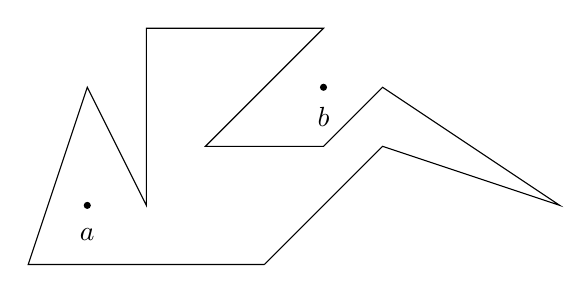
\begin{tikzpicture}[scale=0.75]
%\draw (0,0)--(2,-2)--(3,1)--(5,1)--(2,3)--(1,2)--(-1,2)--(1,4)--(-2,4)--(-2,1)--(-3,3)--(-4,0)--(0,0);
\draw (0,0)--(2,2)--(5,1)--(2,3)--(1,2)--(-1,2)--(1,4)--(-2,4)--(-2,1)--(-3,3)--(-4,0)--(0,0);

\draw[fill] (-3,1) circle [radius=0.05];
\node at (-3,0.5) {$a$};
\draw[fill] (1,3) circle [radius=0.05];
\node at (1,2.5) {$b$};
\end{tikzpicture}
\end{center}

Prikladan način rješavanja zadatka jest
poslati \emph{zraku} iz točke u proizvoljnom smjeru
i izbrojiti koliko puta ona dodiruje
rub mnogokuta.
Ako je taj broj neparan,
točka je unutar mnogokuta,
a ako je broj paran,
točka je izvan mnogokuta.

\begin{samepage}
Na primjer, mogli bismo poslati sljedeće zrake:
\begin{center}
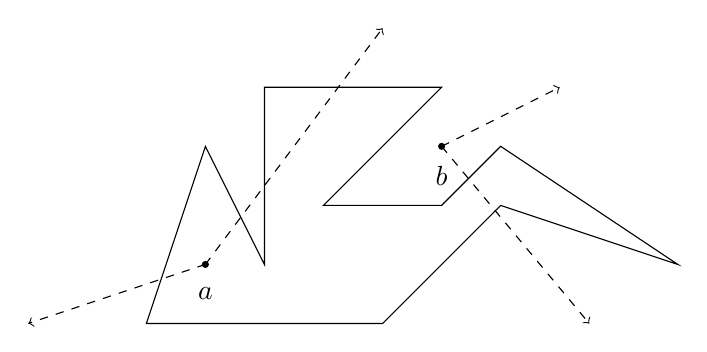
\begin{tikzpicture}[scale=0.75]
\draw (0,0)--(2,2)--(5,1)--(2,3)--(1,2)--(-1,2)--(1,4)--(-2,4)--(-2,1)--(-3,3)--(-4,0)--(0,0);

\draw[fill] (-3,1) circle [radius=0.05];
\node at (-3,0.5) {$a$};
\draw[fill] (1,3) circle [radius=0.05];
\node at (1,2.5) {$b$};

\draw[dashed,->] (-3,1)--(-6,0);
\draw[dashed,->] (-3,1)--(0,5);

\draw[dashed,->] (1,3)--(3.5,0);
\draw[dashed,->] (1,3)--(3,4);
\end{tikzpicture}
\end{center}
\end{samepage}

Zrake iz $a$ dodiruju rub mnogokuta
1 i 3 puta,
pa je $a$ unutar mnogokuta.
Odgovarajuće, zrake iz $b$
dodiruju rub mnogokuta 0 i 2 puta,
pa je $b$ izvan mnogokuta.

\section{Površina mnogokuta}

Opća formula za računanje površine
mnogokuta, koja se ponekad naziva \key{formula vezice},
glasi ovako: \index{formula vezice}
\[\frac{1}{2} |\sum_{i=1}^{n-1} (p_i \times p_{i+1})| =
\frac{1}{2} |\sum_{i=1}^{n-1} (x_i y_{i+1} - x_{i+1} y_i)|, \]
Ovdje su vrhovi
$p_1=(x_1,y_1)$, $p_2=(x_2,y_2)$, $\ldots$, $p_n=(x_n,y_n)$
poredani tako da su
$p_i$ i $p_{i+1}$ susjedni vrhovi na rubu
mnogokuta,
a prvi i posljednji vrh su isti, tj. $p_1=p_n$.

Na primjer, površina mnogokuta
\begin{center}
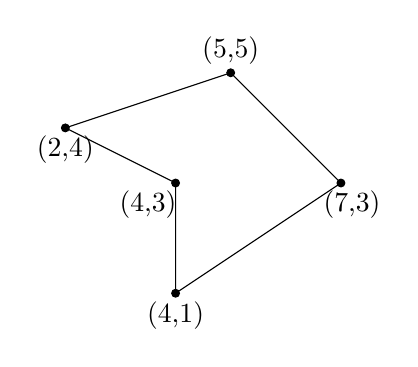
\begin{tikzpicture}[scale=0.7]
\filldraw (4,1.4) circle (2pt);
\filldraw (7,3.4) circle (2pt);
\filldraw (5,5.4) circle (2pt);
\filldraw (2,4.4) circle (2pt);
\filldraw (4,3.4) circle (2pt);
\node (1) at (4,1) {(4,1)};
\node (2) at (7.2,3) {(7,3)};
\node (3) at (5,5.8) {(5,5)};
\node (4) at (2,4) {(2,4)};
\node (5) at (3.5,3) {(4,3)};
\path[draw] (4,1.4) -- (7,3.4) -- (5,5.4) -- (2,4.4) -- (4,3.4) -- (4,1.4);
\end{tikzpicture}
\end{center}
je
\[\frac{|(2\cdot5-5\cdot4)+(5\cdot3-7\cdot5)+(7\cdot1-4\cdot3)+(4\cdot3-4\cdot1)+(4\cdot4-2\cdot3)|}{2} = 17/2.\]

Ideja formule jest proći kroz trapeze
kojima je jedna stranica stranica mnogokuta,
a druga stranica leži na horizontalnom pravcu $y=0$.
Na primjer:
\begin{center}
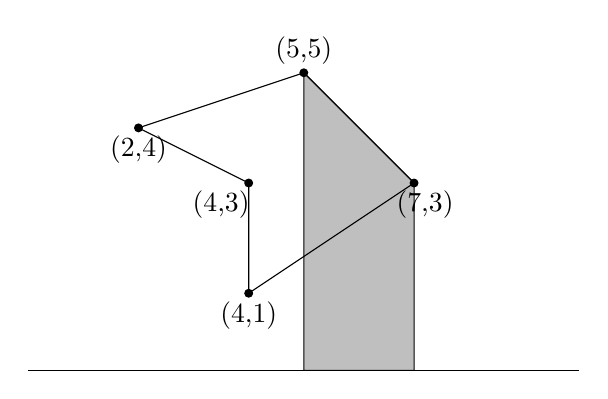
\begin{tikzpicture}[scale=0.7]
\path[draw,fill=lightgray] (5,5.4) -- (7,3.4) -- (7,0) -- (5,0) -- (5,5.4);
\filldraw (4,1.4) circle (2pt);
\filldraw (7,3.4) circle (2pt);
\filldraw (5,5.4) circle (2pt);
\filldraw (2,4.4) circle (2pt);
\filldraw (4,3.4) circle (2pt);
\node (1) at (4,1) {(4,1)};
\node (2) at (7.2,3) {(7,3)};
\node (3) at (5,5.8) {(5,5)};
\node (4) at (2,4) {(2,4)};
\node (5) at (3.5,3) {(4,3)};
\path[draw] (4,1.4) -- (7,3.4) -- (5,5.4) -- (2,4.4) -- (4,3.4) -- (4,1.4);
\draw (0,0) -- (10,0);
\end{tikzpicture}
\end{center}
Površina takvog trapeza je
\[(x_{i+1}-x_{i}) \frac{y_i+y_{i+1}}{2},\]
gdje su vrhovi mnogokuta $p_i$ i $p_{i+1}$.
Ako je $x_{i+1}>x_{i}$, površina je pozitivna,
a ako je $x_{i+1}<x_{i}$, površina je negativna.

Površina mnogokuta je suma površina
svih takvih trapeza, što daje formulu
\[|\sum_{i=1}^{n-1} (x_{i+1}-x_{i}) \frac{y_i+y_{i+1}}{2}| =
\frac{1}{2} |\sum_{i=1}^{n-1} (x_i y_{i+1} - x_{i+1} y_i)|.\]

Uočimo da uzimamo apsolutnu vrijednost sume,
jer vrijednost sume može biti pozitivna ili negativna,
ovisno o tome hodamo li rubom mnogokuta
u smjeru kazaljke na satu ili suprotno od njega.

\subsubsection{Pickov teorem}

\index{Pickov teorem}

\key{Pickov teorem} daje još jedan način računanja
površine mnogokuta uz uvjet da svi vrhovi 
mnogokuta imaju cjelobrojne koordinate.
Prema Pickovom teoremu, površina mnogokuta je
\[ a + b/2 -1,\]
gdje je $a$ broj cjelobrojnih točaka unutar mnogokuta,
a $b$ broj cjelobrojnih točaka na rubu mnogokuta.

Na primjer, površina mnogokuta
\begin{center}
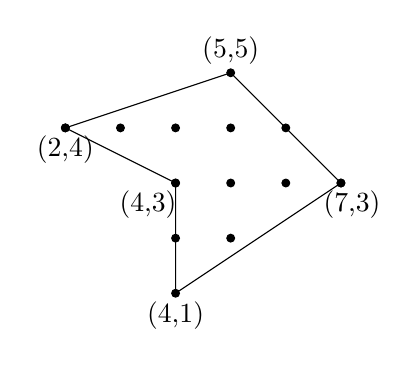
\begin{tikzpicture}[scale=0.7]
\filldraw (4,1.4) circle (2pt);
\filldraw (7,3.4) circle (2pt);
\filldraw (5,5.4) circle (2pt);
\filldraw (2,4.4) circle (2pt);
\filldraw (4,3.4) circle (2pt);
\node (1) at (4,1) {(4,1)};
\node (2) at (7.2,3) {(7,3)};
\node (3) at (5,5.8) {(5,5)};
\node (4) at (2,4) {(2,4)};
\node (5) at (3.5,3) {(4,3)};
\path[draw] (4,1.4) -- (7,3.4) -- (5,5.4) -- (2,4.4) -- (4,3.4) -- (4,1.4);

\filldraw (2,4.4) circle (2pt);
\filldraw (3,4.4) circle (2pt);
\filldraw (4,4.4) circle (2pt);
\filldraw (5,4.4) circle (2pt);
\filldraw (6,4.4) circle (2pt);

\filldraw (4,3.4) circle (2pt);
\filldraw (5,3.4) circle (2pt);
\filldraw (6,3.4) circle (2pt);
\filldraw (7,3.4) circle (2pt);

\filldraw (4,2.4) circle (2pt);
\filldraw (5,2.4) circle (2pt);
\end{tikzpicture}
\end{center}
je $6+7/2-1=17/2$.

\section{Funkcije udaljenosti}

\index{funkcija udaljenosti}
\index{euklidska udaljenost}
\index{Manhattan udaljenost}

\key{Funkcija udaljenosti} definira udaljenost između
dvije točke.
Uobičajena funkcija udaljenosti je
\key{euklidska udaljenost} kod koje je udaljenost između
točaka $(x_1,y_1)$ i $(x_2,y_2)$ jednaka
\[\sqrt{(x_2-x_1)^2+(y_2-y_1)^2}.\]
Alternativna funkcija udaljenosti je
\key{Manhattan udaljenost}
kod koje je udaljenost između točaka
$(x_1,y_1)$ i $(x_2,y_2)$ jednaka
\[|x_1-x_2|+|y_1-y_2|.\]
\begin{samepage}
Na primjer, razmotrimo sljedeću sliku:
\begin{center}
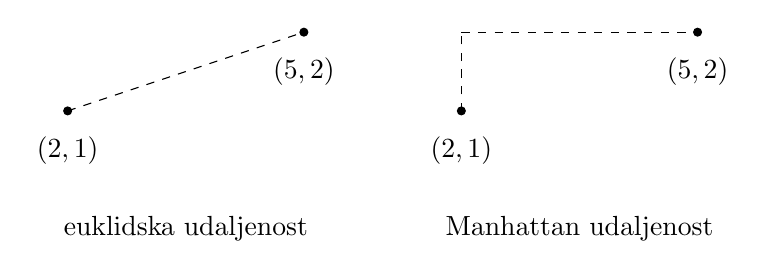
\begin{tikzpicture}

\draw[fill] (2,1) circle [radius=0.05];
\draw[fill] (5,2) circle [radius=0.05];

\node at (2,0.5) {$(2,1)$};
\node at (5,1.5) {$(5,2)$};

\draw[dashed] (2,1) -- (5,2);

\draw[fill] (5+2,1) circle [radius=0.05];
\draw[fill] (5+5,2) circle [radius=0.05];

\node at (5+2,0.5) {$(2,1)$};
\node at (5+5,1.5) {$(5,2)$};

\draw[dashed] (5+2,1) -- (5+2,2);
\draw[dashed] (5+2,2) -- (5+5,2);

\node at (3.5,-0.5) {euklidska udaljenost};
\node at (5+3.5,-0.5) {Manhattan udaljenost};
\end{tikzpicture}
\end{center}
\end{samepage}
Euklidska udaljenost između tih točaka je
\[\sqrt{(5-2)^2+(2-1)^2}=\sqrt{10}\]
a Manhattan udaljenost je
\[|5-2|+|2-1|=4.\]
Sljedeća slika prikazuje područja koja su unutar udaljenosti 1
od središnje točke, uz euklidsku i Manhattan udaljenost:
\begin{center}
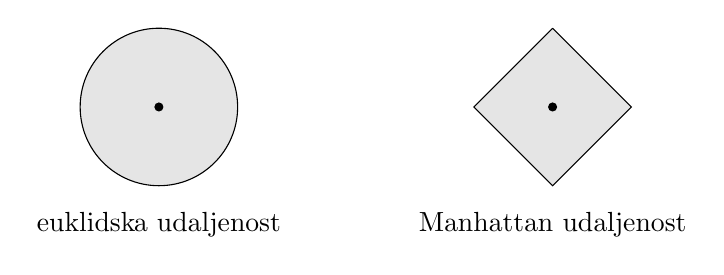
\begin{tikzpicture}

\draw[fill=gray!20] (0,0) circle [radius=1];
\draw[fill] (0,0) circle [radius=0.05];

\node at (0,-1.5) {euklidska udaljenost};

\draw[fill=gray!20] (5+0,1) -- (5-1,0) -- (5+0,-1) -- (5+1,0) -- (5+0,1);
\draw[fill] (5,0) circle [radius=0.05];
\node at (5,-1.5) {Manhattan udaljenost};
\end{tikzpicture}
\end{center}

\subsubsection{Rotiranje koordinata}

Neke je zadatke lakše riješiti ako se
umjesto euklidskih udaljenosti koriste Manhattan udaljenosti.
Kao primjer, razmotrimo zadatak u kojem nam je zadano
$n$ točaka u dvodimenzionalnoj ravnini,
a naš je zadatak izračunati najveću Manhattan
udaljenost između bilo koje dvije točke.

Na primjer, razmotrimo sljedeći skup točaka:
\begin{center}
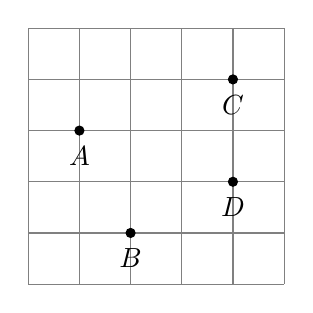
\begin{tikzpicture}[scale=0.65]
\draw[color=gray] (-1,-1) grid (4,4);

\filldraw (0,2) circle (2.5pt);
\filldraw (3,3) circle (2.5pt);
\filldraw (1,0) circle (2.5pt);
\filldraw (3,1) circle (2.5pt);

\node at (0,1.5) {$A$};
\node at (3,2.5) {$C$};
\node at (1,-0.5) {$B$};
\node at (3,0.5) {$D$};
\end{tikzpicture}
\end{center}
Najveća Manhattan udaljenost iznosi 5
i to između točaka $B$ i $C$:
\begin{center}
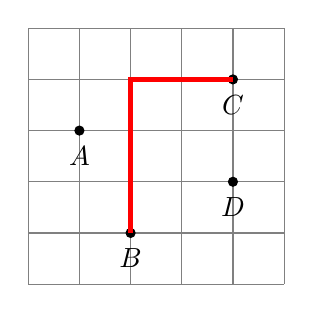
\begin{tikzpicture}[scale=0.65]
\draw[color=gray] (-1,-1) grid (4,4);

\filldraw (0,2) circle (2.5pt);
\filldraw (3,3) circle (2.5pt);
\filldraw (1,0) circle (2.5pt);
\filldraw (3,1) circle (2.5pt);

\node at (0,1.5) {$A$};
\node at (3,2.5) {$C$};
\node at (1,-0.5) {$B$};
\node at (3,0.5) {$D$};

\path[draw=red,thick,line width=2pt] (1,0) -- (1,3) -- (3,3);
\end{tikzpicture}
\end{center}

Korisna tehnika povezana s Manhattan udaljenostima
jest zarotirati sve koordinate za 45 stupnjeva tako da
točka $(x,y)$ postane $(x+y,y-x)$.
Na primjer, nakon rotiranja gornjih točaka
rezultat je:

\begin{center}
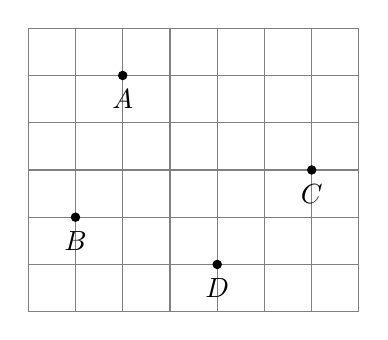
\begin{tikzpicture}[scale=0.6]
\draw[color=gray] (0,-3) grid (7,3);

\filldraw (2,2) circle (2.5pt);
\filldraw (6,0) circle (2.5pt);
\filldraw (1,-1) circle (2.5pt);
\filldraw (4,-2) circle (2.5pt);

\node at (2,1.5) {$A$};
\node at (6,-0.5) {$C$};
\node at (1,-1.5) {$B$};
\node at (4,-2.5) {$D$};
\end{tikzpicture}
\end{center}
A najveća udaljenost je sljedeća:
\begin{center}
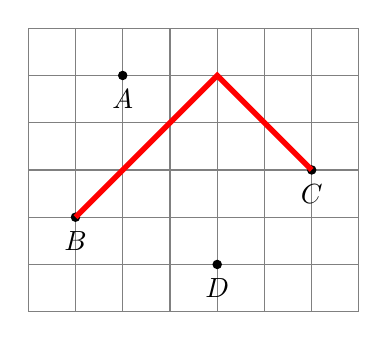
\begin{tikzpicture}[scale=0.6]
\draw[color=gray] (0,-3) grid (7,3);

\filldraw (2,2) circle (2.5pt);
\filldraw (6,0) circle (2.5pt);
\filldraw (1,-1) circle (2.5pt);
\filldraw (4,-2) circle (2.5pt);

\node at (2,1.5) {$A$};
\node at (6,-0.5) {$C$};
\node at (1,-1.5) {$B$};
\node at (4,-2.5) {$D$};

\path[draw=red,thick,line width=2pt] (1,-1) -- (4,2) -- (6,0);
\end{tikzpicture}
\end{center}

Razmotrimo dvije točke $p_1=(x_1,y_1)$ i $p_2=(x_2,y_2)$ čije su
rotirane koordinate $p'_1=(x'_1,y'_1)$ i $p'_2=(x'_2,y'_2)$.
Sada postoje dva načina da izrazimo Manhattan udaljenost
između $p_1$ i $p_2$:
\[|x_1-x_2|+|y_1-y_2| = \max(|x'_1-x'_2|,|y'_1-y'_2|)\]

Na primjer, ako je $p_1=(1,0)$ i $p_2=(3,3)$,
rotirane koordinate su $p'_1=(1,-1)$ i $p'_2=(6,0)$,
a Manhattan udaljenost je
\[|1-3|+|0-3| = \max(|1-6|,|-1-0|) = 5.\]

Rotirane koordinate daju jednostavan način
rada s Manhattan udaljenostima, jer možemo
promatrati x i y koordinate odvojeno.
Da bismo maksimizirali Manhattan udaljenost između dvije točke,
trebamo pronaći dvije točke čije rotirane
koordinate maksimiziraju vrijednost izraza
\[\max(|x'_1-x'_2|,|y'_1-y'_2|).\]
To je jednostavno, jer ili horizontalna ili vertikalna
razlika rotiranih koordinata mora biti najveća.
